\section{SGDW Proyectado}\label{sec:sgdwp}  % MARK: - Section SGDWP

A pesar de que la implementación del SGDW entrega los resultados esperados, el baricentro no parece ser lo suficientemente natural. Por este motivo, se propone una adaptación del SGDW, donde se busca proyectar el baricentro sobre alguna variedad $\Manifold$ de medidas, con el objetivo de hacerlo ver más natural y atractivo.

Para ello, se recapitula la definición de CWB de la Sección~\ref{sec:app-bar-wass-Proyectados}, donde en el trabajo \cite{simon2020barycenters} se explica la forma de proyectar una medida $\mu$ sobre una variedad específica de medidas $\Manifold$, aprendidas por una red generativa.

En este sentido, el conjunto de modelos $\Manifold\subseteq \ProbSpace[\cX] $ correspondería a la variedad generada por la red $G_\theta$, es decir,
\begin{equation}
    \Manifold \eqdef \left\{ G_\theta(z) \in \ProbSpace[\cX] \colon z \in \cZ \right\} \subseteq \ProbSpace[\cX].
\end{equation}
Este cambio puede hacer que el Supuesto~\ref{assump:caso-particular-geodesicamente-convexo} no se cumpla, dado que es posible que $\Manifold$ no sea geodésicamente convexo. Esto provocaría que el Teorema~\ref{thm:convergencia-sgdw} y la Proposición~\ref{prop:convergencia-bsgdw} no garanticen la existencia o la unicidad del baricentro proyectado.



\FM[inline]{Para comprobar estas hipótesis, se realizan los siguientes experimentos.....}
\FM[inline]{Aquí quizás incluir que, por este motivo, se harán experimentos para ver si converge a una única medida o no.}


\subsection{Integración de la Proyección al SGDW}\label{ssec:sgdwp-deduccion-algoritmo}  % MARK: - Integración de la Proyección al SGDW

A pesar de que los autores de \cite{simon2020barycenters} explican que, para obtener los resultados de su artículo utilizan el Algoritmo~\ref{alg:ADMM-CWB}, la realidad es que al revisar su código fuente \cite{imagebar2020simon} se observa que sólo utilizan una iteración del algoritmo anterior (es decir, no utilizan el Lagrangiano Aumentado). De este modo, el algoritmo se simplifica de la siguiente manera: para dos medidas $\mu_0, \mu_1 \in \ProbSpace[\cX] $ y un número $t \in [0, 1]$, empiezan por calcular la $t$-interpolación geodésica de estas medidas (paso 3 del Alg.~\ref{alg:ADMM-CWB}), y luego proyectan este baricentro sobre la variedad $\Manifold$ a través del AE (paso 4 del Alg.~\ref{alg:ADMM-CWB}). El resto de pasos que conciernen al Lagrangiano Aumentado (los pasos 5, 6 y el bucle 2-7) son omitidos en su implementación.

Motivados por esta simplificación, se propone una adaptación del Algoritmo~\ref{alg:sgdw-general} para que proyecte el baricentro en la variedad $\Manifold$, donde además se agrega el parámetro $n_P\in\N$ para proyectar cada $n_P$ iteraciones del algoritmo. De este modo, se deduce el Algoritmo~\ref{alg:sgdwp} para el SGDW Proyectado.
\begin{algorithm}[H]
    \caption{SGDW Proyectado (SGDWP)}
    \label{alg:sgdwp}
    \begin{algorithmic}[1]
        \Require Acceso a las muestras de $\Gamma(\dd \mu) \in \ProbSpace[\ProbSpace]$, un esquema de paso $(\eta_k)_k \in [0, 1]^\N$, un esquema de paso $(S_k)_k \in \N^\N$, un proyector $P:\ProbSpace[\cX] \to \Manifold\subseteq \ProbSpace[\cX] $ y un número $n_P \in \N$.
        \State{$k\gets0$}
        \State{Muestrear $\mu_0 \sim \Gamma$}
        \Repeat
        \State{Muestrear $\tilde \mu_k^{(1)}, \dots, \tilde \mu_k^{(S_k)} \simiid \Gamma$}
        \State{$\gamma\gets\qty(1-\eta_k, \frac{\eta_k}{S_k}, \dots, \frac{\eta_k}{S_k})$}
        \State Definir $\mu_k$ como el baricentro de $\qty( \mu_k, \tilde\mu_k^{(1)}, \dots, \tilde\mu_k^{(S_k)} )$ con pesos $\gamma$.
        \If{$k \mod n_P = 0$}
        \State{$\mu_k\gets P(\mu_k)$}\Comment{Proyectar $\mu_k$ sobre $\Manifold$}
        \EndIf
        \State{$k\gets k+1$}
        \Until{un criterio de detención ha sido alcanzado.}
        \State{$\mu_k\gets P(\mu_k)$}\Comment{Terminar con una última proyección antes de retornar.}
        \State\Return $\mu_k$
    \end{algorithmic}
\end{algorithm}

\FM[inline]{Este párrafo podría ser parte de las conclusiones? Onda, por el trabajo futuro.}

Cabe destacar que el Algoritmo~\ref{alg:sgdwp} tiene una mecánica similar al Método del Gradiente Proyectado (MPG)~\cite[Secc. 5.1]{optimizacion2022amaya}, puesto que este es un método de optimización con restricciones que, si en una iteración se viola alguna restricción, entonces se proyecta dicha iteración sobre el conjunto de restricciones. Este es el caso del Algoritmo~\ref{alg:sgdwp}, donde se proyecta el baricentro en la variedad $\Manifold$. Sin embargo, se diferencia del MPG, en que el dominio $\Manifold$ puede no ser (geodésicamente) convexo.

\FM[inline]{debería mencionar como se implemnetó el proyector $P$ en más detalle?}

\subsection{Experimentos}\label{ssec:sgdwp-experimentos}  % MARK: - Experimentos

\subsubsection{Único Baricentro}\label{sssec:sgdwp-unico-bar}  % MARK: - Único Baricentro


Una primera pregunta que se tiene es:
\begin{quotation}
    \centering
    ¿Existe un único baricentro para este problema?
\end{quotation}
% ¿existe un único baricentro para este problema? 
Como se sabe, y los experimentos de la Sección~\ref{sec:sgdw} corroboraron, el baricentro que computa el SGDW es único y consistente. Sin embargo, la variedad $\Manifold$ en este caso puede no ser geodésicamente convexa, por lo que no se puede garantizar la unicidad del baricentro proyectado. Por este motivo, para saber si existe alguna convergencia en el baricentro proyectado, se ejecuta el Algoritmo~\ref{alg:sgdwp} múltiples veces para observar los distintos resultados, y verificar si son similares o no.

Para este experimento, se utiliza el mismo esquema $(\eta_k)_k$ de la Ecuación~\ref{eq:esquema-paso}, usando los mismos parámetros mencionados. Para el esquema de lotes, se utiliza $S_k=1,\ \forall k \in \N$. Para definir el proyector, se utilizan las redes neuronales planteadas en la Capítulo~\ref{chap:WAE-WGAN}, de manera que el proyector se definiría por $P = \ProbQ_\varphi (G_\theta (\bullet))$\FM{Quizás comentar en la sección de la WGAN-WAE que se hará el abuso de notación cuando se asume que $\ProbQ$ es determinista.}. Además se fija $n_P=1$ para proyectar en cada iteración del algoritmo.

El resultado de este experimento se puede observar en la Figura~\ref{fig:bar-SGDWP-exp}, donde se muestran los baricentros proyectados obtenidos en diez experimentos distintos. Se puede observar que los baricentros proyectados son distintos entre sí, lo que sugiere que no existe un único baricentro proyectado para este problema.
\begin{figure}[H]
    \centering
    % Experimento 01
    \begin{subfigure}[b]{0.17\textwidth}
        \centering
        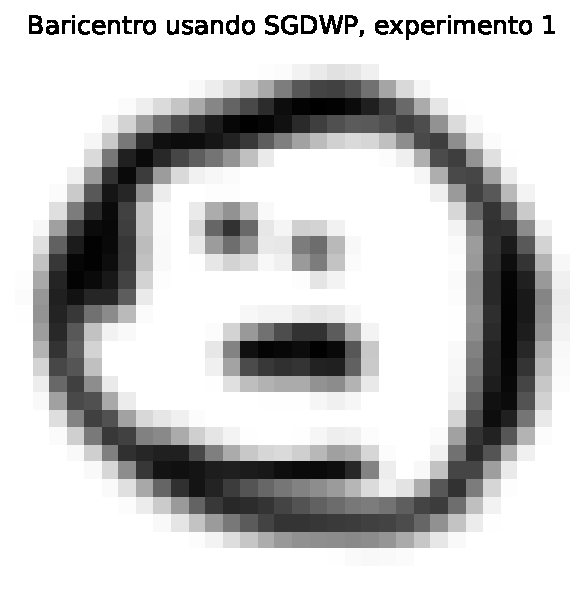
\includegraphics[width=\textwidth]{img/sgdwp/bar-SGDWP-exp-01.pdf}
        % \caption{}
        \label{fig:bar-SGDWP-exp-01}
    \end{subfigure}
    \hfill
    % Experimento 02
    \begin{subfigure}[b]{0.17\textwidth}
        \centering
        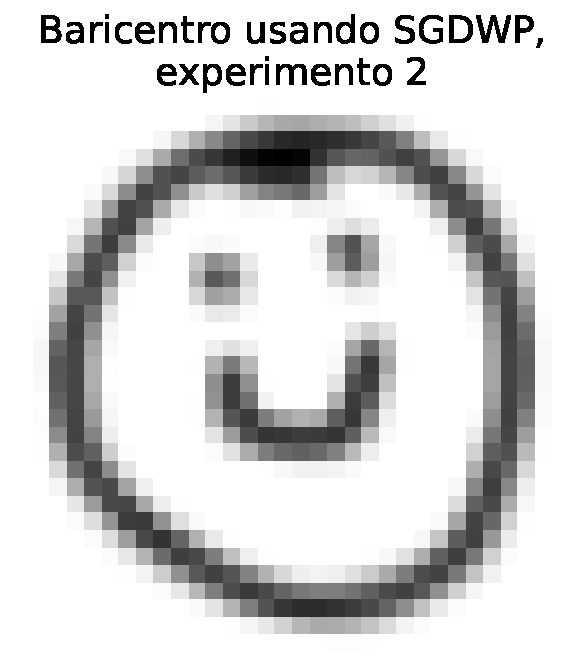
\includegraphics[width=\textwidth]{img/sgdwp/bar-SGDWP-exp-02.pdf}
        % \caption{}
        \label{fig:bar-SGDWP-exp-02}
    \end{subfigure}
    \hfill
    % Experimento 03
    \begin{subfigure}[b]{0.17\textwidth}
        \centering
        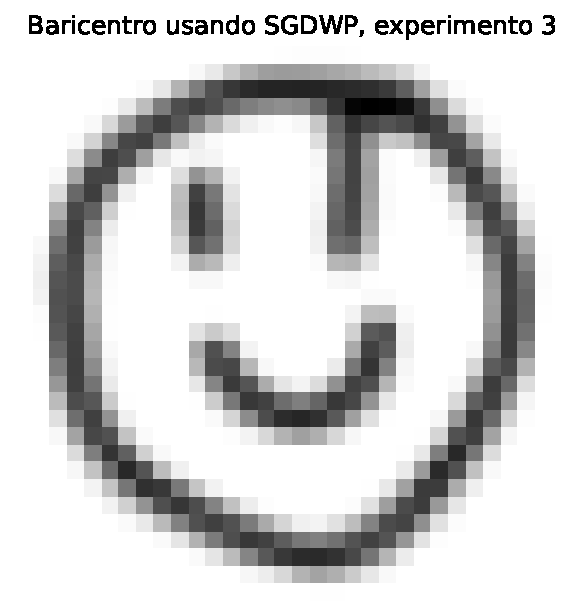
\includegraphics[width=\textwidth]{img/sgdwp/bar-SGDWP-exp-03.pdf}
        % \caption{}
        \label{fig:bar-SGDWP-exp-03}
    \end{subfigure}
    \hfill
    % Experimento 04
    \begin{subfigure}[b]{0.17\textwidth}
        \centering
        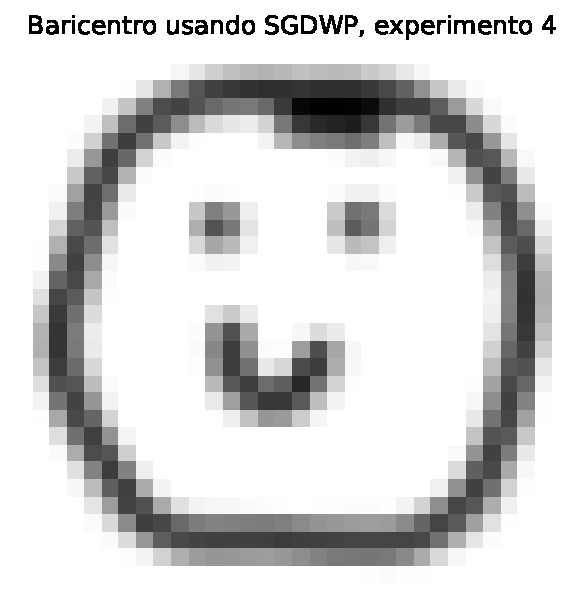
\includegraphics[width=\textwidth]{img/sgdwp/bar-SGDWP-exp-04.pdf}
        % \caption{}
        \label{fig:bar-SGDWP-exp-04}
    \end{subfigure}
    \hfill
    % Experimento 05
    \begin{subfigure}[b]{0.17\textwidth}
        \centering
        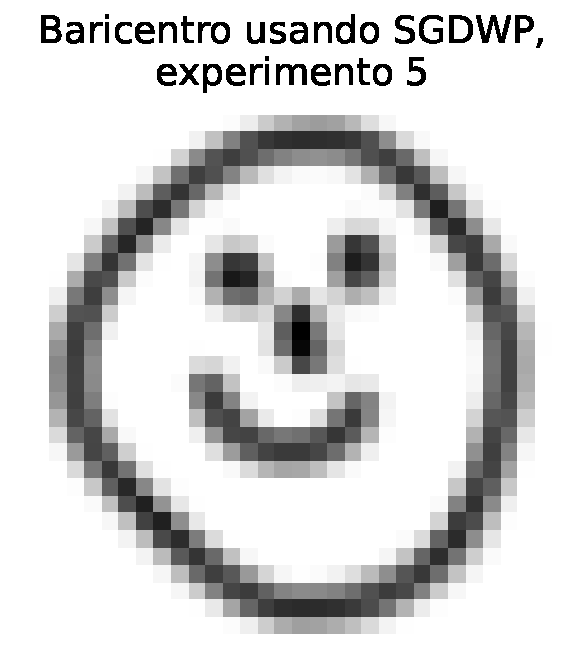
\includegraphics[width=\textwidth]{img/sgdwp/bar-SGDWP-exp-05.pdf}
        % \caption{}
        \label{fig:bar-SGDWP-exp-05}
    \end{subfigure}
    \newline
    % Experimento 06
    \begin{subfigure}[b]{0.17\textwidth}
        \centering
        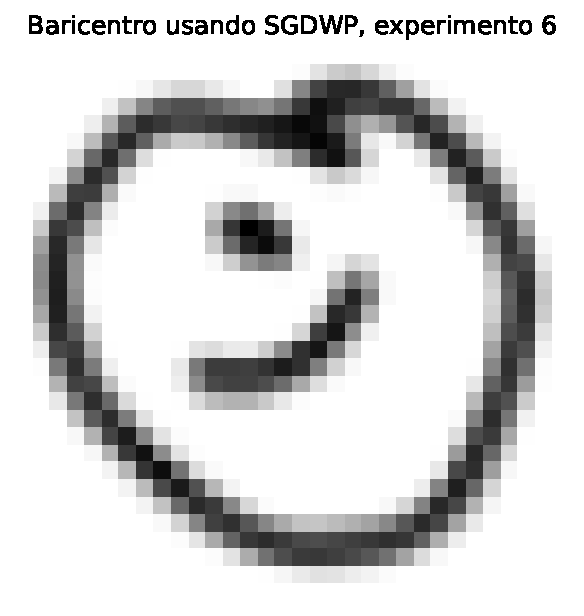
\includegraphics[width=\textwidth]{img/sgdwp/bar-SGDWP-exp-06.pdf}
        % \caption{}
        \label{fig:bar-SGDWP-exp-06}
    \end{subfigure}
    \hfill
    % Experimento 07
    \begin{subfigure}[b]{0.17\textwidth}
        \centering
        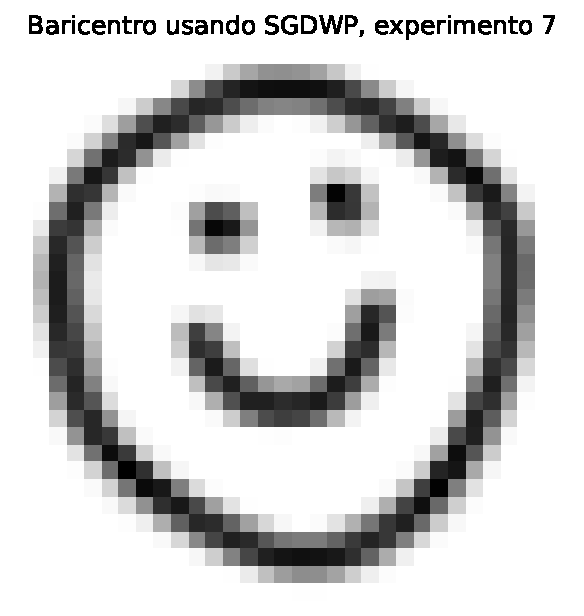
\includegraphics[width=\textwidth]{img/sgdwp/bar-SGDWP-exp-07.pdf}
        % \caption{}
        \label{fig:bar-SGDWP-exp-07}
    \end{subfigure}
    \hfill
    % Experimento 08
    \begin{subfigure}[b]{0.17\textwidth}
        \centering
        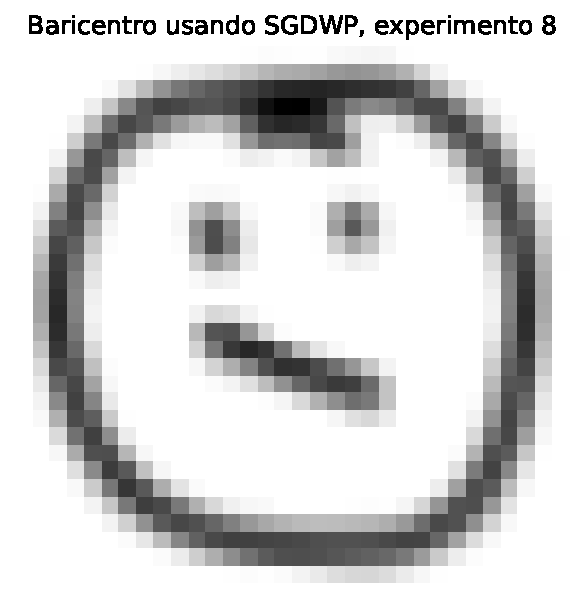
\includegraphics[width=\textwidth]{img/sgdwp/bar-SGDWP-exp-08.pdf}
        % \caption{}
        \label{fig:bar-SGDWP-exp-08}
    \end{subfigure}
    \hfill
    % Experimento 09
    \begin{subfigure}[b]{0.17\textwidth}
        \centering
        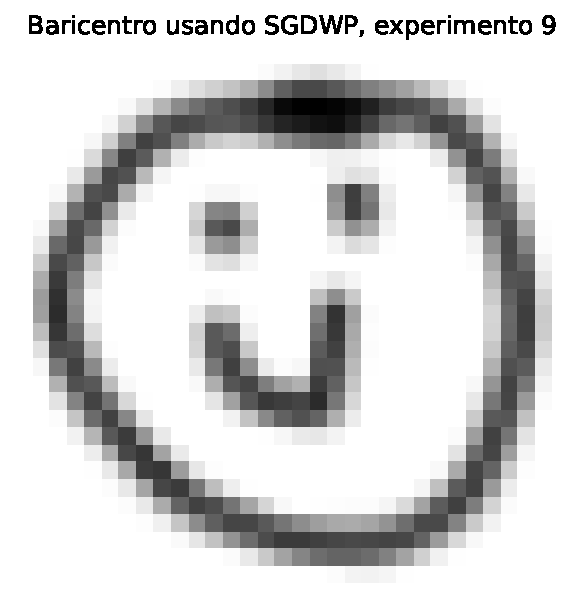
\includegraphics[width=\textwidth]{img/sgdwp/bar-SGDWP-exp-09.pdf}
        % \caption{}
        \label{fig:bar-SGDWP-exp-09}
    \end{subfigure}
    \hfill
    % Experimento 10
    \begin{subfigure}[b]{0.17\textwidth}
        \centering
        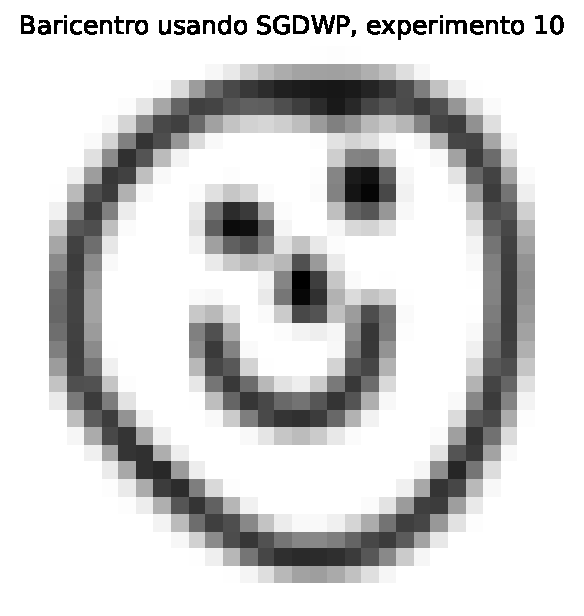
\includegraphics[width=\textwidth]{img/sgdwp/bar-SGDWP-exp-10.pdf}
        % \caption{}
        \label{fig:bar-SGDWP-exp-10}
    \end{subfigure}
    \caption{Baricentros proyectados obtenidos por el Algoritmo~\ref{alg:sgdwp} en diez experimentos distintos.}
    \label{fig:bar-SGDWP-exp}
\end{figure}

\subsubsection{Variando el Parámetro de Proyectar Cada}\label{sssec:sgdwp-variar-param}  % MARK: - Variando el Parámetro de Proyectar Cada

Otra pregunta que surge es:
\begin{quotation}
    \centering
    ¿Cómo afecta el parámetro $n_P$ en la convergencia del baricentro proyectado?
\end{quotation}
Una hipótesis que se tiene es que permitir que se den algunas iteraciones del algoritmo ``clásico'' permitirá tener una mejor estimación del baricentro original antes de proyectarlo en la variedad $\Manifold$. Para verificar esta hipótesis, se ejecuta el Algoritmo~\ref{alg:sgdwp} con distintos valores de $n_P$ y se observa cómo afecta en la convergencia del baricentro proyectado.

En particular, se ejecutará con los valores $n_P \in \left\{ 1, 3, 5, 10 \right\}$.

\begin{figure}[htbp]
    \centering
    \begin{subfigure}[b]{0.23\textwidth}
        \centering
        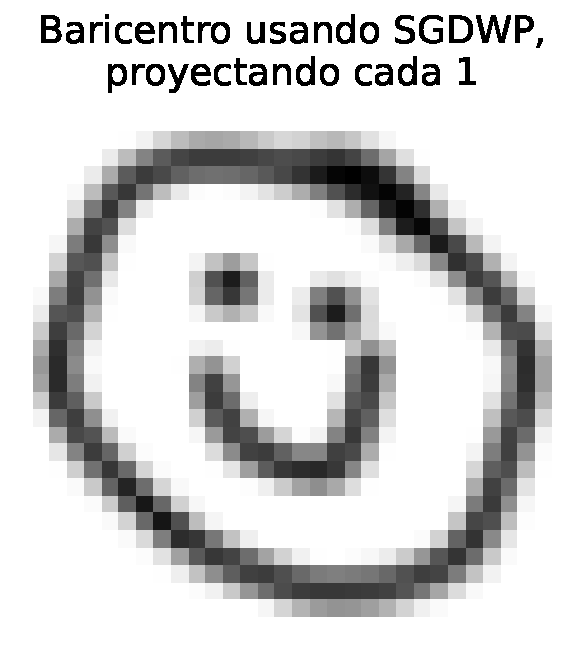
\includegraphics[width=\textwidth]{img/sgdwp-pe/bar-SGDWP-pe-01.pdf}
        \caption{$n_P=1$}
        \label{fig:bar-SGDWP-pe-01}
    \end{subfigure}
    \hfill
    \begin{subfigure}[b]{0.23\textwidth}
        \centering
        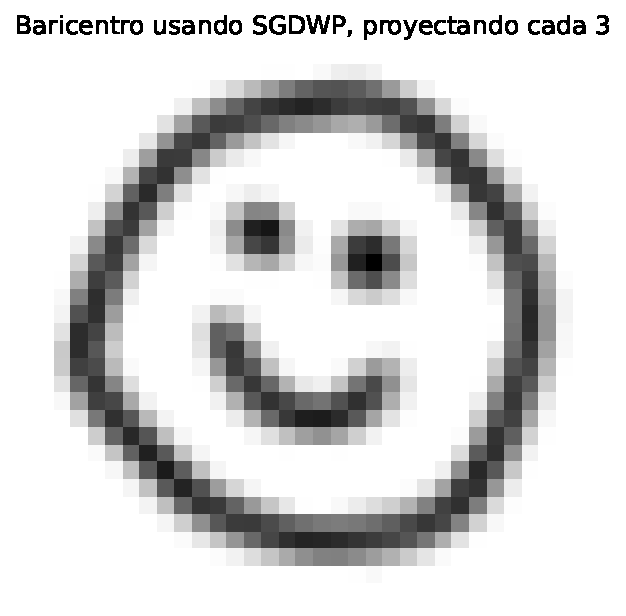
\includegraphics[width=\textwidth]{img/sgdwp-pe/bar-SGDWP-pe-03.pdf}
        \caption{$n_P=3$}
        \label{fig:bar-SGDWP-pe-03}
    \end{subfigure}
    % \newline
    \hfill
    \begin{subfigure}[b]{0.23\textwidth}
        \centering
        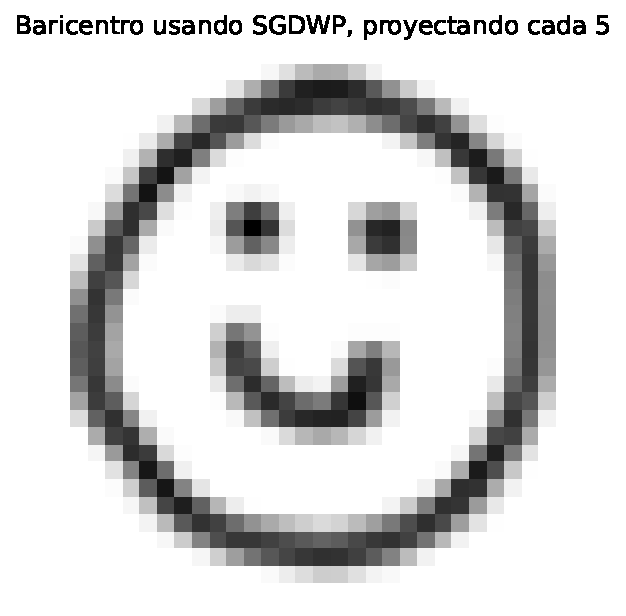
\includegraphics[width=\textwidth]{img/sgdwp-pe/bar-SGDWP-pe-05.pdf}
        \caption{$n_P=5$}
        \label{fig:bar-SGDWP-pe-05}
    \end{subfigure}
    \hfill
    \begin{subfigure}[b]{0.23\textwidth}
        \centering
        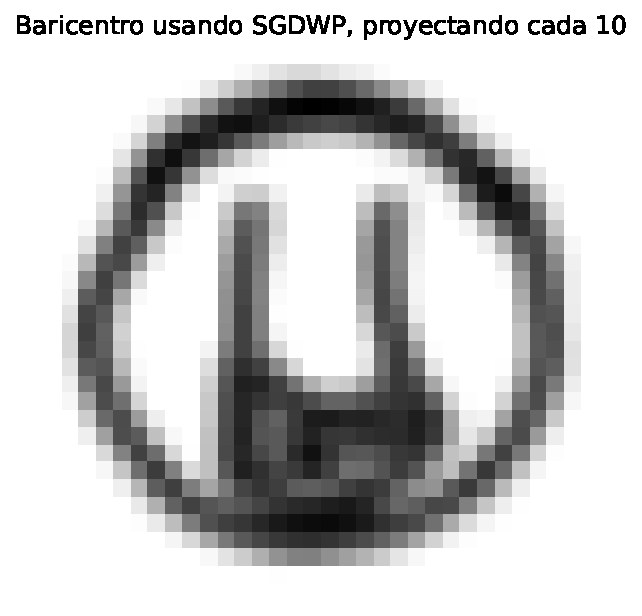
\includegraphics[width=\textwidth]{img/sgdwp-pe/bar-SGDWP-pe-10.pdf}
        \caption{$n_P=10$}
        \label{fig:bar-SGDWP-pe-10}
    \end{subfigure}
    % \includegraphics[width=0.5\textwidth]{}
    \caption{Baricentros proyectados obtenidos por el Algoritmo~\ref{alg:sgdwp} con distintos valores de $n_P$.}
    \label{fig:bar-SGDWP-pe}
\end{figure}

En el Anexo~\ref{anx:sgdwp} se presentan las iteraciones por las que pasaron estos baricentros.




\subsection{Resultados y Discusión}\label{ssec:sgdwp-resultados-discusion}  % MARK: - Resultados y Discusión



\subsection{Conclusiones}\label{ssec:sgdwp-conclusiones}  % MARK: - Conclusiones

